\section{PACT}\label{sec:PACT}
This Section is unless anything else is stated based upon \cite{Benyon}.

When designing an interactive system it is important to be human-centered, since it is the users who at the end determines the use of a given system.
\\\indent
Depending on how well designers have implemented a way to convey their conception of a given system, different users will interpret it differently. 
Their interpretation, being based on individual understanding and knowledge, regulates the users interactions with the system and thereby determines what it really does, see \cref{fig:PACT-SystemImage}.

\begin{figure}[H]
	\centering
	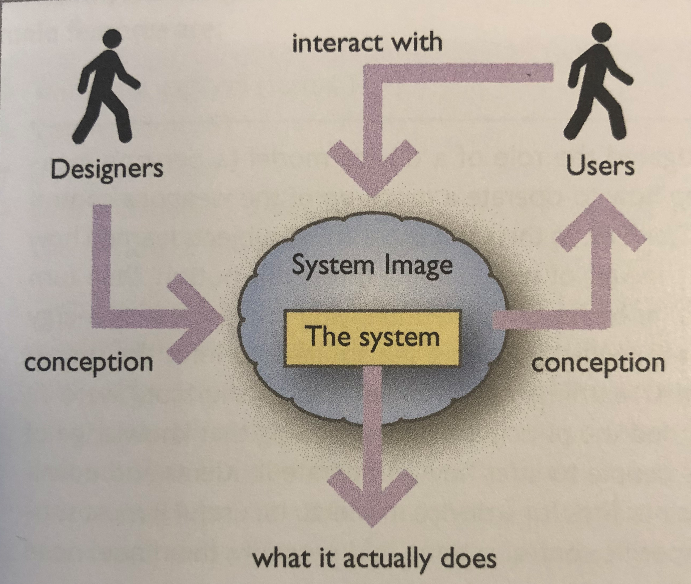
\includegraphics[width=0.5\textwidth]{billeder/SystemImage-Benyon.png}
	\caption{\textit{The System Image from {\color{red}Benyon side 31}}}
	\label{fig:PACT-SystemImage}
\end{figure}

To help understand and reflect upon the users and their relation to a interactive system, the framework PACT is used. 
PACT is an acronym for ''people, activities, contexts and technologies'', see \cref{sec:PACT-method} for further details.
This analysis framework is used to analyze the users, such that developers are able to design the system people-centered instead of machine-centered.
%The method also helps developers to reflect upon how to best convey their conception and the essence of the system to the users and thereby influence users interactions with the system.

\subsection{The acronym outlined}\label{sec:PACT-method}
\subsubsection*{People}
People differs from each others in many ways.
This element in the PACT analysis is a way to ponder upon these differences as well as a way to categorize the different users of a system. 
Three differences usually discussed in this part of the analysis is:
\begin{itemize}
	\item Physiological
	\item Psychological
	\item Social
\end{itemize}

\textbf{Physiological differences} covers the relevant ways people differs in physical characteristics.
This could be, differences in perception from the five senses; sight, hearing, touch, smell and taste as well along with age, height or weight.
\begin{example} 
As an example, when making an interface it is important to consider color blindness, since it affects about $8\%$ men and $0.5\%$ women in the world \cite{ColourBlind}.
\end{example}

\textbf{Psychological differences} describes things such as; emotional make-up, how stress affects different people, attention, memory and spatial ability.
Furthermore, is language and culture also important points to consider since these affect the psyche and thereby the way people interpret things.
\begin{example}
	In USA is a tick used when marking acceptance and a cross to mark rejection, while it in Britain can be used for both. Brits do among other use a cross on the voting paper.
\end{example}


\textbf{Social differences} is about how people use system for different reasons and therefore can have various goals. 
Additionally, there is also a big difference in people expertise levels which affects how an interface might be designed.
\\\indent
This is an important consideration since designing a system for a homogeneous group of people is  distinct from designing one for a heterogeneous group.

\subsubsection*{Activities}

\subsubsection*{Contexts}

\subsubsection*{Technologies}






































\subsection{PACT analysis}\label{sec:PACT-analysis}
Based on the interview
\todo{maybe interviews depending on whether or not we change it after further interviews}
with Pia,
% conslutant and acting quality chief at JBJ,
{\color{red} section XX}, the PACT analysis for the project described in this report is as follows.

\subsubsection*{People}

There are four main groups of people; the quality manager, the secretary, department heads and everyday workers.
This is a heterogeneous group with different levels of IT experience ranging from no skills with IT and therefore cautious about it, to the level of everyday office work.
The group also has different levels of domain expertise ranging from no to expert which needs to be considered. The quality manager is a domain expert and therefore has different needs of the system than the everyday worker with no expertise.
\newline
Furthermore, issues such as colorblindness, other eye handicap as well as bad memory need to be considered when designing the system and interface.


\subsubsection*{Activities}
The overall activities is to manage, update and access a handbook mostly the newest version but also possibly older versions as well. It is needed to uphold the standards from the government to retain the companies certifications.
This is a well defined activity
which takes place at least yearly, though sometimes more often.
%In the case of JBJ it happens more often
When doing the activities users may experience interruptions and should therefore be simple to use and easy to get back to.
Additionally, the activities is mostly done alone but may be done in collaboration with others, though this is not required.
\newline
The data to be entered into the system are mostly larger data entries and possibly many of such.
the system is not safety critical but integrity is an important aspect.

\subsubsection*{Contexts}


\subsubsection*{Technologies}














